\documentclass{article}
\usepackage[utf8]{inputenc}
\usepackage[english]{babel}
\usepackage{amsmath} 
\usepackage{amsthm}
\usepackage{amsfonts}
\usepackage{graphicx}

\graphicspath{ {images/} }

\newtheorem{theorem}{Theorem}

\theoremstyle{definition}
\newtheorem{definition}{Definition}
\theoremstyle{definition}
\newtheorem{example}{Example}

\begin{document}

\title{Spherical Harmonics: Approximating Functions With Orthogonal Bases}
\author{Justin Meiners}

\maketitle

\section{Introduction}

In this paper I will explain how to use sets of simple functions as a basis for approximating more complicated functions. This is similar to trigonometric fourier series but more general. Along the way I will explain how the theory applies to functions on the unit sphere called spherical harmonics. At the end I will apply this theory to a problem in computer graphics.

\section{Inner Products}

In analysis we generalized the notion of distance by definining a metric, which as an operator with certain properties that ensure it acts like a "distance function". For example, it would not make sense to talk about negative distances, so a metric must always be positive.

We can similarly generalize the idea of a dot product by definining an inner product in terms of its essential properties.

\begin{definition}
    An \textbf{inner product} is binary operation with the following properties:

    Let $x, y, z\in V$ and $a\in R$

    \begin{enumerate}
        \item Positive definite: $\langle x, x\rangle=0$ when $x=0$ otherwise $\langle x, x \rangle>0$
        \item Symmetric: $\langle x, y \rangle=\langle y, x \rangle$.
        \item Linear: $\langle ax, y \rangle= a\langle x, y \rangle$.
        \item Distributive: $\langle x, y + z \rangle = \langle x, y \rangle + \langle x, z \rangle$
    \end{enumerate}
\end{definition}

\begin{example}
    Since we wanted to generalize dot product, we expect the euclidean dot product to satisfy these properties.

    $$\langle x, y \rangle =\sum_{i=1}^{n} x_{i}y_{i}$$
\end{example}

\begin{example} 
    The topic of this paper is approximating functions. What might an inner product of functions look like? We can think of it as a continuous dot product. The dot product is the sum of multiples of each vector component. Given two functions $f(x), g(x)$ we can similarly add up multiples of their values at every point. This is of course an integral.

    $$\langle f(x), g(x) \rangle = \int_{a}^{b} f(x)g(y) dx$$
    This is an inner product of integrable functions on the interval $[a, b]$.
\end{example}

\begin{example}
    Later we will be approximating functions on the unit sphere. This requires a more exotic inner product which is a spherical integral.

    $$\langle f(\theta, \phi), g(\theta, \phi) \rangle=\int_{0}^{2\pi}\int_{0}^{\pi}f(\theta, \phi)g(\theta, \phi)\sin\phi\ \partial\phi \partial\theta$$

\end{example}


\subsection{Inner Product Spaces}

The presence of an inner product gives us more structure than a plain vector space. 

\begin{definition}
    An \textbf{inner product space} is a vector space with an inner product operation.
\end{definition}


\section{Orthogonal Systems}

As we know from euclidean geometry that vectors $x, y$ are said to be orthogonal when $\langle x, y \rangle$=0. This term also applies to any inner product space.

\begin{example}
    What does this look like for functions? An example of two orthogonal functions is $\cos(\pi x)$ and $\cos(2\pi x)$. The image on the right highlights the inner product which makes it easier to see what is happening.

    \begin{figure}[h]
        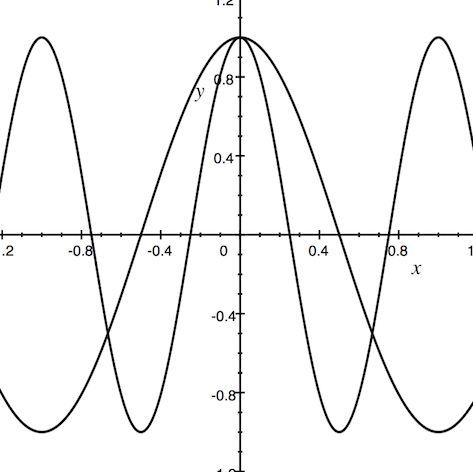
\includegraphics[scale=0.3]{ortho}
        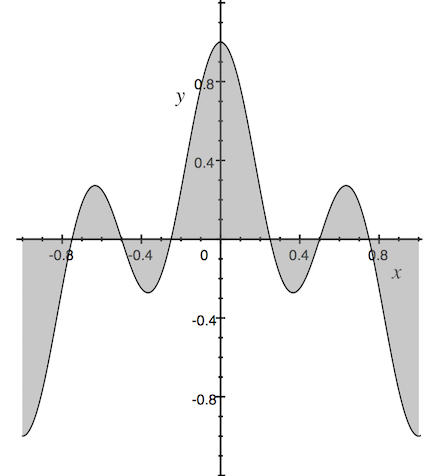
\includegraphics[scale=0.3]{ortho-int}
        \centering
    \end{figure}
\end{example}


\begin{definition}
    A set $\{u_{1}, u_{2}, \ldots, u_{n} \}$ is called an \textbf{orthogonal system} iff for each $i,j\in \{ 1 \ldots n \}$  $\langle u_{i}, u_{j} \rangle=0$ whenever $i\neq j$.

\end{definition}
Informally it is a set of vectors in which each vector is orthogonal to every other vector in the set.

\subsection{Linear Independance}

\begin{theorem}
    The vectors in an orthogonal system are linearly independant
\end{theorem}

\begin{proof}
    Suppose $c_{1}u_{1}+c_{2}u_{2}+\ldots+c_{n}u_{n}=0$

    Let $i\in \{ 1...n \}$. Then:
    \begin{equation}
        \begin{split}
            &\langle u_{i}, c_{1}u_{1} + c_{2}u_{2} + \ldots + c_{n}u_{n} \rangle \\ 
            &= \langle u_{i}, c_{1}u_{1} \rangle + \langle u_{i}, c_{2}u_{2} \rangle + \ldots + \langle u_{i}, c_{i}u_{i} \rangle + \ldots + \langle u_{i}, c_{n}u_{n} \rangle \\
            &= c_{1}\langle u_{i}, u_{1} \rangle + c_{2}\langle u_{i}, u_{2} \rangle + \ldots + c_{i}\langle u_{i}, u_{i} \rangle + \ldots + c_{n}\langle u_{i}, u_{n} \rangle \\
            &= c_{i}\langle u_{i}, u_{i} \rangle=0 
        \end{split}
    \end{equation}

    Since $\langle u_{i}, u_{i} \rangle \neq 0$ then $c_{i}=0$.
    Therefore the set is linearly independant.
\end{proof}

\subsection{Completeness}

Linear independance leads us to think about forming a basis for our vector space. Specifically to approximate functions, we want to create a basis for our space of functions. We now know we can create a linearly indepedant set from orthogonal vectors, for a finite set this guarentee's the vectors span, but not for an infinite space.

\begin{definition}
    An orthogonal system $S$ is said to be \textbf{complete} iff the smallest space containing $S$ is the whole inner product space $R$.
\end{definition}

Completeness is always relative to the space. Clearly an orthogonal system is always complete in some space (the span of the vectors).

\begin{definition}
    An orthogonal system which is complete is called an \textbf{orthogonal basis}.
\end{definition}

\begin{example}
    The standard basis vectors are an orthgonal basis for $\mathbb{R}^{n}$ under the dot product.
    \begin{equation}
        \begin{split}
            e_{1}&=( 1, 0, \ldots, 0 ) \\
            e_{2}&=( 0, 1, \ldots, 0 ) \\
            \ldots \\
            e_{n}&=( 0, 0, \ldots, 1 ) 
        \end{split}
    \end{equation}
\end{example}

\begin{example}
    The powers of x are an orthogonal basis for the space of real polynomials.
     $$S=\{ 1, x, x^{2}, x^{3}, \ldots, x^{n}, \ldots \}$$
\end{example}

\begin{example}
    Laplace's equation states
    $$\nabla\cdot\nabla f=0$$.

    Although the derivation is significant\cite{laplace-equation} 3D spherical coordinates this can be written as:

    $$\frac{\partial^{2}}{\partial r^{2}}+\frac{2}{r}\frac{\partial}{\partial r} + \frac{1}{r^{2}\sin^{2}(\phi)}\frac{\partial^{2}}{\partial \theta^{2}}+\frac{1}{r^{2}}\frac{\partial^{2}}{\partial \phi^{2}}+\frac{\cot(\phi)}{r^{2}}\frac{\partial}{\partial \phi}=0$$

    The \textbf{spherical harmonics} are functions which satisfy this equation. They form an orthogonal basis for the space of integrable functions on the unit sphere, using the spherical inner product introduced earlier.

    $$Y_{\ell}^{m}(\theta, \phi)=\sqrt{\frac{(2\ell +1)(\ell-m)!}{4\pi(\ell+m)!}}P_{\ell}^{m}(\cos\phi)e^{im\theta}$$

    Where $P_{\ell}^{m}$ are the associated legendre polynomials.
\end{example}

\section{Bessel's Inequality}

We will now explore Bessel's inequality which will tell us when an orthogonal system is complete. In this section we will refer to the norm of a vector. We will not explore the definition or properties of vector spac enorms here. For our usage the norm is defined by the following:

\begin{definition}
    $||x||=\sqrt{\langle x, x \rangle}$
\end{definition}

\begin{definition}
    Let $U=\{u_{1}, u_{2}, \ldots \}$ be an orthogonal system and $x\in R$ where $R$ is an inner product space. Define the coordinates $c_{i}$ with respect to $U$ as $c_{i}=\langle u_{i}, x \rangle$.
\end{definition}

\begin{theorem}
    Let $U=\{u_{1}, u_{2}, \ldots \}$ be an orthonormal system and $x\in R$. Then: 
    $$||x - \sum_{i=1}^{\infty} a_{i}u_{i}||$$
    Is minimized when $a_{i}=c_{i}$, the coordinates with respect to $U$.
\end{theorem}

In other words linear combinations of the vectors in the orthogonal system get closest to the function when they are scaled by the coordintaes.

\begin{proof}
    \begin{equation}
    \begin{split}
        ||x - \sum_{i=1}^{\infty} a_{i}u_{i}||^{2}&=\langle x - \sum_{i=1}^{\infty} a_{i}u_{i}, x - \sum_{i=1}^{\infty} a_{i}u_{i} \rangle \\
        &= \langle x, x \rangle - 2\langle x, \sum_{i=1}^{\infty} a_{i}u_{i} \rangle + \langle \sum_{i=1}^{\infty} a_{i}u_{i}, \sum_{i=1}^{\infty} a_{i}u_{i} \rangle \\
        &= ||x||^{2} - 2\sum_{i=1}^{\infty} a_{i}c_{i} + \sum_{i=1}^{\infty} a_{i}^{2}||u_{i}||^{2} \\
        &= ||x||^{2} - 2\sum_{i=1}^{\infty} a_{i}c_{i} + \sum_{i=1}^{\infty} a_{i}^{2} + \sum_{i=1}^{\infty} (c_{i}^{2} - c_{i}^{2}) \\
        &= ||x||^{2} + (\sum_{i=1}^{\infty} a_{i}^{2} - 2\sum_{i=1}^{\infty} a_{i}c_{i} + \sum_{i=1}^{\infty} c_{i}^{2}) - \sum_{i=1}^{\infty} c_{i}^{2} \\
        &= ||x||^{2} + \sum_{i=1}^{\infty} (a_{i} - c_{i})^{2} - \sum_{i=1}^{\infty} c_{i}^{2} 
    \end{split}
    \end{equation}
   
    This is smallest when the middle term drops out which is when $a_{i} = c_{i}$.
\end{proof}

\begin{theorem}
    Bessel's Inequality
    $$\sum_{i=1}^{\infty}c_{i}^{2} \leq ||x||^{2}$$
\end{theorem}

\begin{proof}
    \begin{equation}
    \begin{split}
        \langle x - \sum_{i=1}^{\infty} a_{i}u_{i}, x - \sum_{i=1}^{\infty} a_{i}u_{i} \rangle &\geq 0 \\
        ||x||^{2} + \sum_{i=1}^{\infty} (a_{i} - c_{i})^{2} - \sum_{i=1}^{\infty} c_{i}^{2} &\geq 0 \\
        ||x||^{2} - \sum_{i=1}^{\infty} c_{i}^{2} &\geq 0 \\
        ||x||^{2} &\geq \sum_{i=1}^{\infty} c_{i}^{2}
    \end{split}
    \end{equation} 
\end{proof}


\begin{theorem}
    An orthogonal system is complete iff Bessel's Inequality is always equal.
\end{theorem}

\begin{proof}
    We want to show that any vector $x$ in $V$ is equal to linear combinations of the basis elements. In other words the basis spans $V$.
    \begin{equation}
    \begin{split}
        ||x - \sum_{i=1}^{\infty} c_{i}u_{i}||^{2}&=||x||^{2} + \sum_{i=1}^{\infty} (c_{i} - c_{i})^{2} - \sum_{i=1}^{\infty} c_{i}^{2} = 0 \\
        x=\sum_{i=1}^{\infty} c_{i}u_{i} \\
    \end{split}
    \end{equation}
\end{proof}

So to prove that an orthogonal system is complete we only need to verify that Bessel's inequality is an equality.

\section{Application}
In computer graphics, each object in the scene must be lit directly from each light source (radiance), as well as by light which is bounced from the surronding scene (irradiance). Since light is incoming from all directions, this effect can be modeled as function on a sphere $f(\theta, \phi)$. The normal vectors on the surface of the model are used to evaluate the function to calculate the color value at each point on the surface.

\begin{figure}[h]
    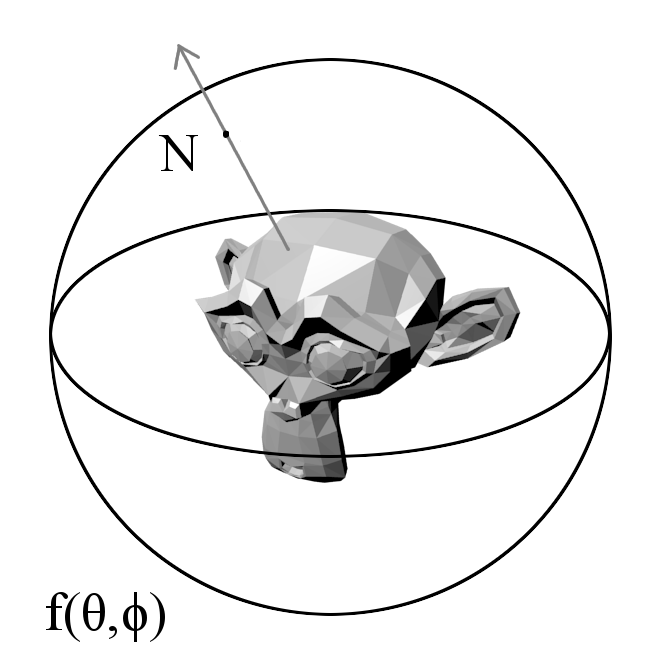
\includegraphics[scale=0.35]{sphere-function}
    \centering
\end{figure}

Unfortunatly, storing this incoming light function, over the entire sphere is not trivial. A common techniques is to place light probes around the scene. At each probe a set of 6 images is rendered (up, down, left, right, forward, back). Nearby objects then  a cubemap (a set of 6 images in a cube) is rendered of the sorrounding scene and then evalatuted. This provides high quality lighting but requires a significant amount of memory to store each of these images.

\begin{figure}[h]
    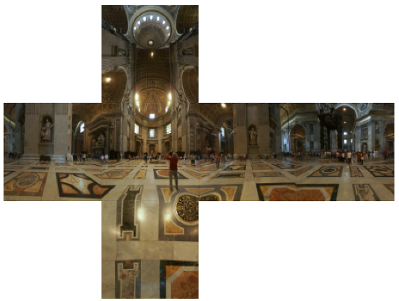
\includegraphics[scale=0.30]{cubemap}
    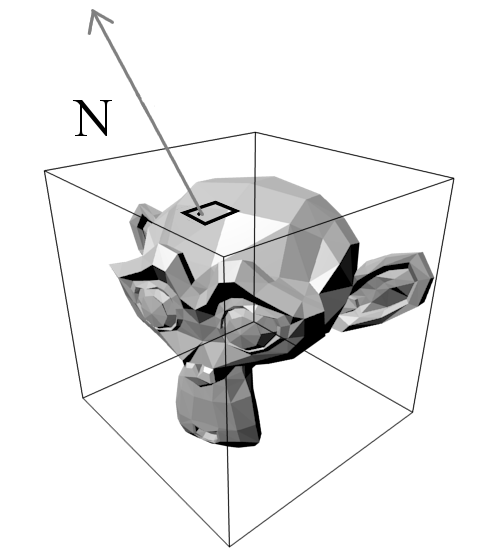
\includegraphics[scale=0.35]{cube-function}
    \centering
\end{figure}

With the theory we have just developed we can do better by approximating the lighting function using the orthgonal basis of the spherical harmonics. For very reflective materials, such as metal, an image is necessary to capture high frequency detail, but most materials need a lower frequency signal. For common materials we need only the first 9 spherical harmonics to get a good approximation. \cite{sh-lighting}

\subsection*{Preprocess Step}
\begin{enumerate}
    \item At each probe in the scene render 6 images of the surrounding enviornment to create a cubemap. We will denote each color channel of the cubemap by the function $g_{\alpha}(\theta, \phi)$ where $\alpha\in \{R, G, B \}$.
    \item For each $\alpha$ calculate the 9 coeffecients $s_{\ell}^{m}$ using the inner product.
        $$s_{\ell}^{m}=\langle Y_{\ell}^{m}(\theta, \phi), g_{\alpha}(\theta, \phi) \rangle=
        \int_{0}^{2\pi}\int_{0}^{\pi} Y_{\ell}^{m}(\theta, \phi) g_{\alpha}(\theta, \phi) \sin\phi\ \partial\phi \partial\theta$$
        For $0\leq\ell\leq2$ and $-\ell\leq m \leq\ell$.
\end{enumerate}

\subsection*{Rendering Step}
\begin{enumerate}
    \item Find the closest probe to this model and get its 9 coeffecients.
    \item For each pixel or vertex
        \begin{enumerate}
            \item Calculate the approximate lighting value using the coeffecients and the spherical harmonic functions.
                $$x_{\alpha}=\sum_{\ell=0}^{2} \sum_{m=-\ell}^{\ell} s_{\ell}^{m}Y_{\ell}^{m}(\theta, \phi)$$ 

        \end{enumerate}
\end{enumerate}

Additional details can be found in Ramamoorthi \cite{sh-lighting} and Green \cite{sh-gritty}.

\subsection*{Results}

The following images were captured from my implementation of this method. The original cubemap is shown on the left, with the spherical harmonic approximation on the right.

\begin{figure}[h]
    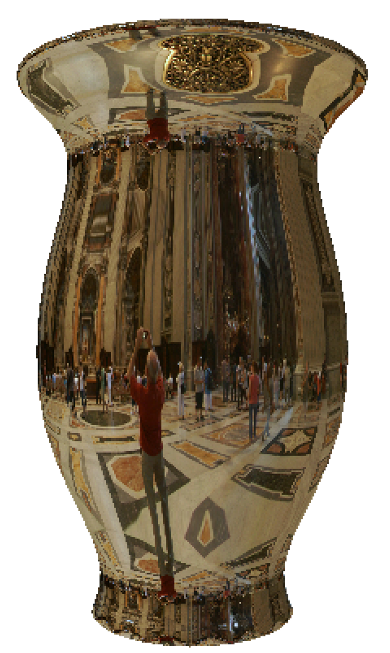
\includegraphics[scale=0.25]{vase2}
    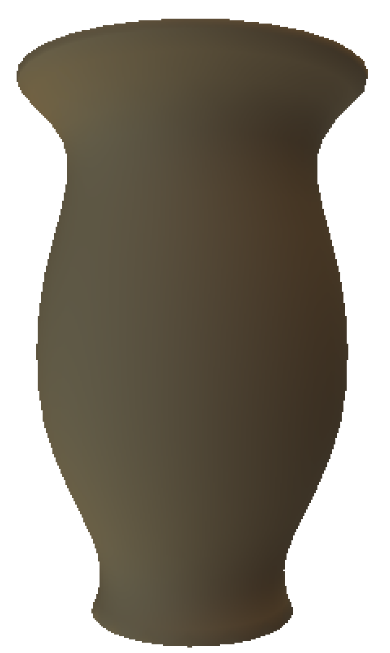
\includegraphics[scale=0.25]{vase2-sh}
    \centering
\end{figure}

\begin{figure}[h]
    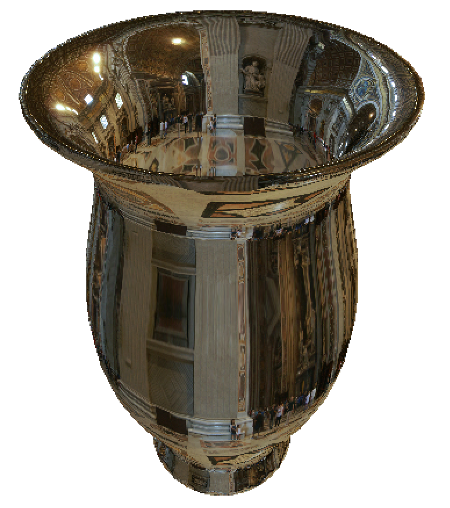
\includegraphics[scale=0.25]{vase1}
    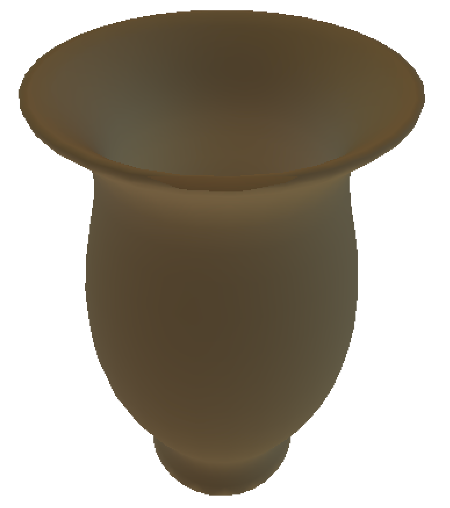
\includegraphics[scale=0.25]{vase1-sh}
    \centering
\end{figure}

\pagebreak

\begin{thebibliography}{999}

\bibitem{intro-analysis}
  A.N Kolmogorov \& S.V. Fomin,
  \emph{Introductory Real Analysis}.
  Dover Books,
\bibitem{laplace-equation}
    Justin Meiners,
   \emph{Deriving Laplace's Equation in Spherical Coordinates}
\bibitem{sh-lighting}
    Ravi Ramamoorthi \& Pat Hanrahan,
    \emph{An Efficient Representation for Irradiance Enviornment Maps}
\bibitem{sh-gritty}
    Robin Green
    \emph{Spherical Harmonic Lighting: The Gritty Details},
    Sony Computer Entertainment America
\bibitem{cubemap}
    Cubemap images were taken from: http://www.humus.name/

\end{thebibliography}

\end{document}
